%%%%%%%%%%%%%%%%%%%%%%%%%%%%%%%%%%%%%%%%%
% CSE 4316/4317 Sprint Report Template
% Version 1.0 (2/18/2018)
% Author: Christopher D. McMurrough
%%%%%%%%%%%%%%%%%%%%%%%%%%%%%%%%%%%%%%%%%

%----------------------------------------------------------------------------------------
%	PACKAGES AND DOCUMENT CONFIGURATIONS
%----------------------------------------------------------------------------------------

\documentclass{article}
\usepackage{siunitx}
\usepackage{graphicx}
\usepackage{amsmath}
\setlength\parindent{0pt}

\usepackage[letterpaper, portrait, margin=1in]{geometry}

%----------------------------------------------------------------------------------------
%	DOCUMENT SECTIONS
%----------------------------------------------------------------------------------------

% report title
\title{Sprint 1 Report \\ CSE 4316}

% author name
\author{Ellen Ripley}

% date of assignment submission
\date{January 1st, 2024}

\begin{document}
\maketitle
\begin{center}
\begin{tabular}{l r}

% sprint start date
Sprint start date: & December 9th, 2023 \\

% sprint end date
Sprint end date: & December 26th, 2023 \\

% project title
Project title: & Awesome Robot System \\

% team name
Team name: & The Roboticists \\

% team members
Partners: 	& Tony Stark \\
			& Sarah Connor \\
			& Alex Murphy \\
        	& Kyle Reese \\
Instructor: & Christopher D. McMurrough
\end{tabular}
\end{center}

% sprint goal
\section{Sprint Goal}
Completion of robotic platform integration tasks in preparation for future ground testing

% sprint backlog
\section{Sprint Backlog}
Breakdown of planned tasks assigned to team (work units expressed in hours). \\ % work units do not have to be hours, change text accordingly

% ADD OR REMOVE ROWS FROM THE TABLE AS NECESSARY (DO NOT LEAVE BLANK ROWS!)
\begin{tabular}{| p{4in} | >{\centering\arraybackslash} p{1in} | >{\centering\arraybackslash} p{1in} |}
\hline
\textbf{Task description} & \textbf{Estimated work} & \textbf{Actual work} \\ \hline
Description of task 1 (add/remove rows as necessary) & 1.0 & 1.0 \\ \hline
Description of task 2 & 1.0 & 1.0 \\ \hline
Description of task 3 & 1.0 & 1.0 \\ \hline
Description of task 4 & 1.0 & 1.0 \\ \hline
Description of task 5 & 1.0 & 1.0 \\ \hline
Description of task 6 & 1.0 & 1.0 \\ \hline
Description of task 7 & 1.0 & 1.0 \\ \hline
Description of task 8 & 1.0 & 1.0 \\ \hline
Description of task 9 & 1.0 & 1.0 \\ \hline
Description of task 10 & 1.0 & 1.0 \\ \hline
\textbf{TOTAL} & \textbf{15.0}  & \textbf{15.0} \\ \hline
\end{tabular}

\pagebreak

% individual time summary
\section{Individual Time Expenditures}
Summary of tasks (planned or unplanned) performed by the individual (work units expressed in hours) \\ % work units do not have to be hours, change text accordingly

% ADD OR REMOVE ROWS FROM THE TABLE AS NECESSARY (DO NOT LEAVE BLANK ROWS!)
% PERCENT COMPLETE DESCRIBES THE STATE OF THE TASK AS OF THE LAST SPRINT DAY (WAS IT FINISHED? IF NOT, APPROXIMATELY HOW "COMPLETE" IS THE TASK)
\begin{tabular}{| p{4in} | >{\centering\arraybackslash} p{1in} | >{\centering\arraybackslash} p{1in} |}
\hline
\textbf{Task Description} & \textbf{Actual work} & \textbf{Percent complete} \\ \hline
Description of task 1 (add/remove rows as necessary) & 1.0 & 100\% \\ \hline
Description of task 2 & 1.0 & 100\% \\ \hline
Description of task 3 & 1.0 & 100\% \\ \hline
Description of task 4 & 1.0 & 50\% \\ \hline
Description of task 5 & 1.0 & 50\% \\ \hline
\textbf{TOTAL} & \textbf{5.0}  & \textbf{-} \\ \hline
\end{tabular}

% burndown chart
\section{Team Burndown Chart}
Burndown chart showing day-to-day progress on sprint tasks. Ideal (baseline) daily effort and actual daily effort of the team are both shown in the figure below.
\begin{figure}[h]
\begin{center}
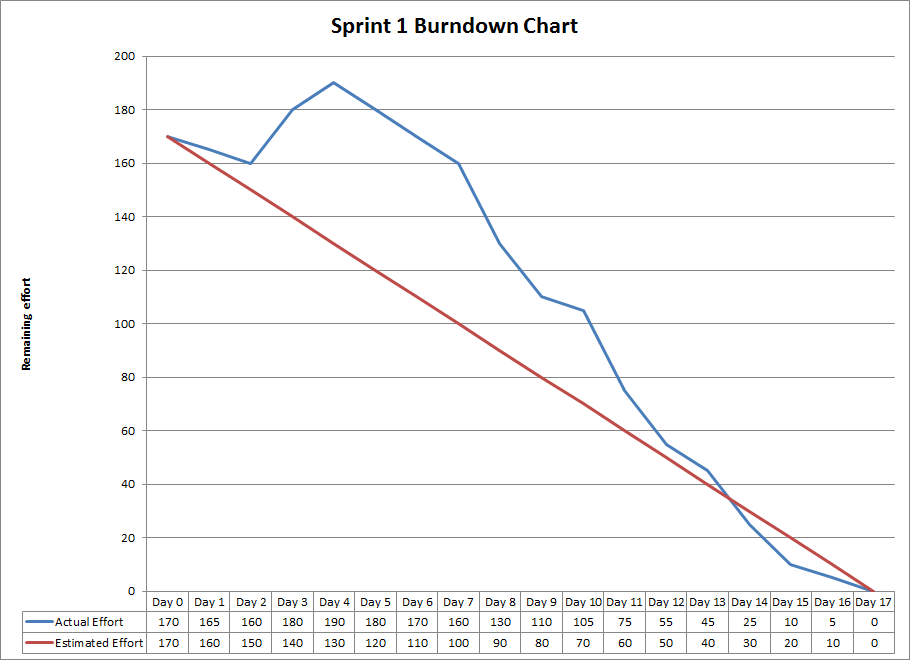
\includegraphics[width=1.0\textwidth]{burndown} % Include the image burndown.png
\end{center}
\end{figure}

\pagebreak

%individual sprint retrospective
\section{Individual Retrospective}
The following lists describe actions (as an individual) that will be started, stopped, or continued during the next sprint to maximize work efficiency. \\

Actions and/or items to \textbf{start} doing in the next sprint (top 3)
\begin{itemize}
\begin{item}
Description of first item
\end{item}
\begin{item}
Description of second item
\end{item}
\begin{item}
Description of third item
\end{item}
\end{itemize}

Actions and/or items to \textbf{stop} doing in the next sprint (top 3)
\begin{itemize}
\begin{item}
Description of first item
\end{item}
\begin{item}
Description of second item
\end{item}
\begin{item}
Description of third item
\end{item}
\end{itemize}

Actions and/or items to \textbf{continue} doing in the next sprint (top 3)
\begin{itemize}
\begin{item}
Description of first item
\end{item}
\begin{item}
Description of second item
\end{item}
\begin{item}
Description of third item
\end{item}
\end{itemize}


%peer review
\section{Peer Review}
Provide a review for each individual team member's performance during this sprint, including yourself. This assessment should be your own candid opinion, and your response will not be shared with other team members. Each item should be assigned a numeric grade of 1-5, where 1 is the lowest possible score and 5 is the highest. \\

Evaluation items:
\begin{itemize}
\begin{item}
Participation - Was the team member present during meetings, work sessions, or any other planned team activities? Were they involved in establishing goals and planning tasks? Did they actively contribute to the development of the project? 
\end{item}
\begin{item}
Communication - Did the team member provide timely updates on progress or challenges faced? Did they use any official team communication technologies effectively? 
\end{item}
\begin{item}
Work quality - Was the team member willing to claim tasks from the backlog? Did the team member meet their objectives? Did the work reported by the team member provide added value to the project? If bugs were present or features were skipped, how severe was the negative impact? 
\end{item}
\begin{item}
Professionalism - Did the team member conduct themselves in a way that would generally be acceptable in a professional work environment while participating in team activities? Did they provide any leadership on tasks? Did they take part in creating a collaborative and inclusive environment? Are they taking the project seriously?
\end{item}
\begin{item}
Overall - How valuable overall was this team member to the project during this evaluation period? You may consider factors not covered in other evaluation items. A score of 1 means that, in your opinion, this individual deserves to be fired.
\end{item}
\end{itemize}

\begin{tabular}{| p{1.5in} | >{\centering\arraybackslash} p{1.in} | >{\centering\arraybackslash} p{1.1in} | >{\centering\arraybackslash} p{1.1in}| >{\centering\arraybackslash} p{0.5in}| >{\centering\arraybackslash} p{.5in} |}
\hline
\textbf{Team member name} & \textbf{Participation} & \textbf{Communication} & \textbf{Professionalism} & \textbf{Work quality} & \textbf{Overall} \\ \hline
Ellen Ripley & 5 & 5 & 5 & 5 & 5\\ \hline
Tony Stark & 2 & 2 & 4 & 3 & 3\\ \hline
Sarah Connor & 3 & 3 & 5 & 5 & 4\\ \hline
Alex Murphy & 5 & 5 & 2 & 3 & 4\\ \hline
Kyle Reese & 4 & 4 & 4 & 5 & 4\\ \hline
\end{tabular}

\end{document}
